%!TEX program = xelatex
\documentclass[xcolor={table},show notes]{beamer}
\usepackage[space]{grffile}
%\setbeameroption{show only notes}

\usepackage[english]{babel}	
\usepackage[utf8]{inputenc}
\usepackage[T1]{fontenc}
\usepackage[scaled]{helvet}
\usepackage{amsthm}
\usepackage{ragged2e}
\usepackage{subfig}
\usepackage[table]{xcolor}
\usepackage{multicol}
\usepackage{multirow}
\usepackage{fancyvrb}
\usepackage{verbatim}
\usepackage{graphicx}
\usepackage{tikz}
\usepackage{booktabs} % For professional looking tables
\usepackage{multirow}
\usepackage{color, colortbl}
\usepackage[table]{xcolor}
\setlength{\aboverulesep}{0pt}
\setlength{\belowrulesep}{0pt}
%\usepackage{multicol}
%\usepackage{longtable}
\usepackage{tabularx}

\usepackage{biblatex}
\addbibresource{references.bib}
\tikzset{
	invisible/.style={opacity=0},
	visible on/.style={alt=#1{}{invisible}},
	alt/.code args={<#1>#2#3}{%
		\alt<#1>{\pgfkeysalso{#2}}{\pgfkeysalso{#3}} % \pgfkeysalso doesn't change the path
	},
}
\usepackage{pgfplots}
\usetikzlibrary{positioning}
\usetikzlibrary{fit}
\usetikzlibrary{backgrounds}
\usetikzlibrary{calc}
\usetikzlibrary{shapes}
\usetikzlibrary{mindmap}
\usetikzlibrary{decorations.text}
\pgfplotsset{compat=1.7}
\usetheme{Execushares}
\setbeamercovered{transparent=15}
\newcommand<>{\uncovergraphics}[2][{}]{
	% Taken from: <https://tex.stackexchange.com/a/354033/95423>
	\begin{tikzpicture}
	\node[anchor=south west,inner sep=0] (B) at (4,0)
	{\includegraphics[#1]{#2}};
	\alt#3{}{%
		\fill [draw=none, fill=ExecusharesWhite, fill opacity=0.7] (B.north west) -- (B.north east) -- (B.south east) -- (B.south west) -- (B.north west) -- cycle;
	}
	\end{tikzpicture}
}






\title{Machine learning for ecosystem
assessment in the Amazon, using
environmental DNA data}
\subtitle{In Collaboration with NatureMetrics}
\author{Adamos Spanashis}
\date{September 17, 2019}

\setcounter{showSlideNumbers}{1}

\begin{document}
	\setcounter{showProgressBar}{0}
	\setcounter{showSlideNumbers}{0}

	\frame{\titlepage}

	\begin{frame}
		\frametitle{Contents}
		\begin{enumerate}
			\item Motivation \\ \textcolor{ExecusharesGrey}{\footnotesize\hspace{1em} Why we applied machine learning}
			\item Data \\ \textcolor{ExecusharesGrey}{\footnotesize\hspace{1em} Our data set; features and class labels}
			\item Train-Validation-Test\\ \textcolor{ExecusharesGrey}{\footnotesize\hspace{1em} How we evaluated the classifiers}
			\item Results \\ \textcolor{ExecusharesGrey}{\footnotesize\hspace{1em} Results of the project}
		\end{enumerate}
	\end{frame}

	\setcounter{framenumber}{0}
	\setcounter{showProgressBar}{1}
	\setcounter{showSlideNumbers}{1}
	\section{Motivation}
		\begin{frame}
			\frametitle{Why monitor the environment}
		\setbeamerfont{itemize/enumerate body}{size = \Large}
			
{		
	
		\begin{itemize}
				\item Rising human populations.
				\pause
				\item Increase in unmanaged waste, especially running waters.
				\pause
				\item Assessment of environmental health developed as a response. 
			\end{itemize}
		
	}
		\end{frame}

		\begin{frame}
			\frametitle{\LARGE Traditional environmental monitoring}
			\begin{itemize}
				\item Selecting indicator species associated with specific kind of pollution.
				\pause
				\item Morpho-taxonomic identification of organisms.
				\pause
				\item Filling up biotic indices to quantify pollution.
			\end{itemize}
		\end{frame}
	\begin{frame}
	\frametitle{\LARGE Traditional monitoring disadvantages}
	\begin{itemize}
		\item Taxonomic identification requires experts, is time consuming and expensive.
		\pause
		\item Selection of indicator species is arbitrary.
		\pause
		\item Taxonomic resolution is low.
	\end{itemize}
	\end{frame}
	\begin{frame}
\frametitle{\LARGE Traditional monitoring disadvantages}
\begin{columns}
	\column{0.5\textwidth}
	\begin{center}
	\includegraphics[width=\textwidth]{Chironomus_plumosus_MHNT}
	Chironomus Plumosus
	\end{center}
	\column{0.5\textwidth}
	\begin{center}
		\includegraphics[width=\textwidth]{chironomus_zealandicus__common_midge-2}
		Chironomus Zealandicus
	\end{center}
\end{columns}
\end{frame}
\begin{frame}
\frametitle{\LARGE Genomics; A new hope?}
\only<1,3->{ \begin{itemize}
	\item<1-> Sanger Sequencing 1977
	
	\item<3-> Barcoding and taxonomic reference libraries
	
	\item<4-> Next Generation Sequencing 
	
	\item<5-> Costs go down by orders of magnitude  
\end{itemize}}
\only<2>{\centering
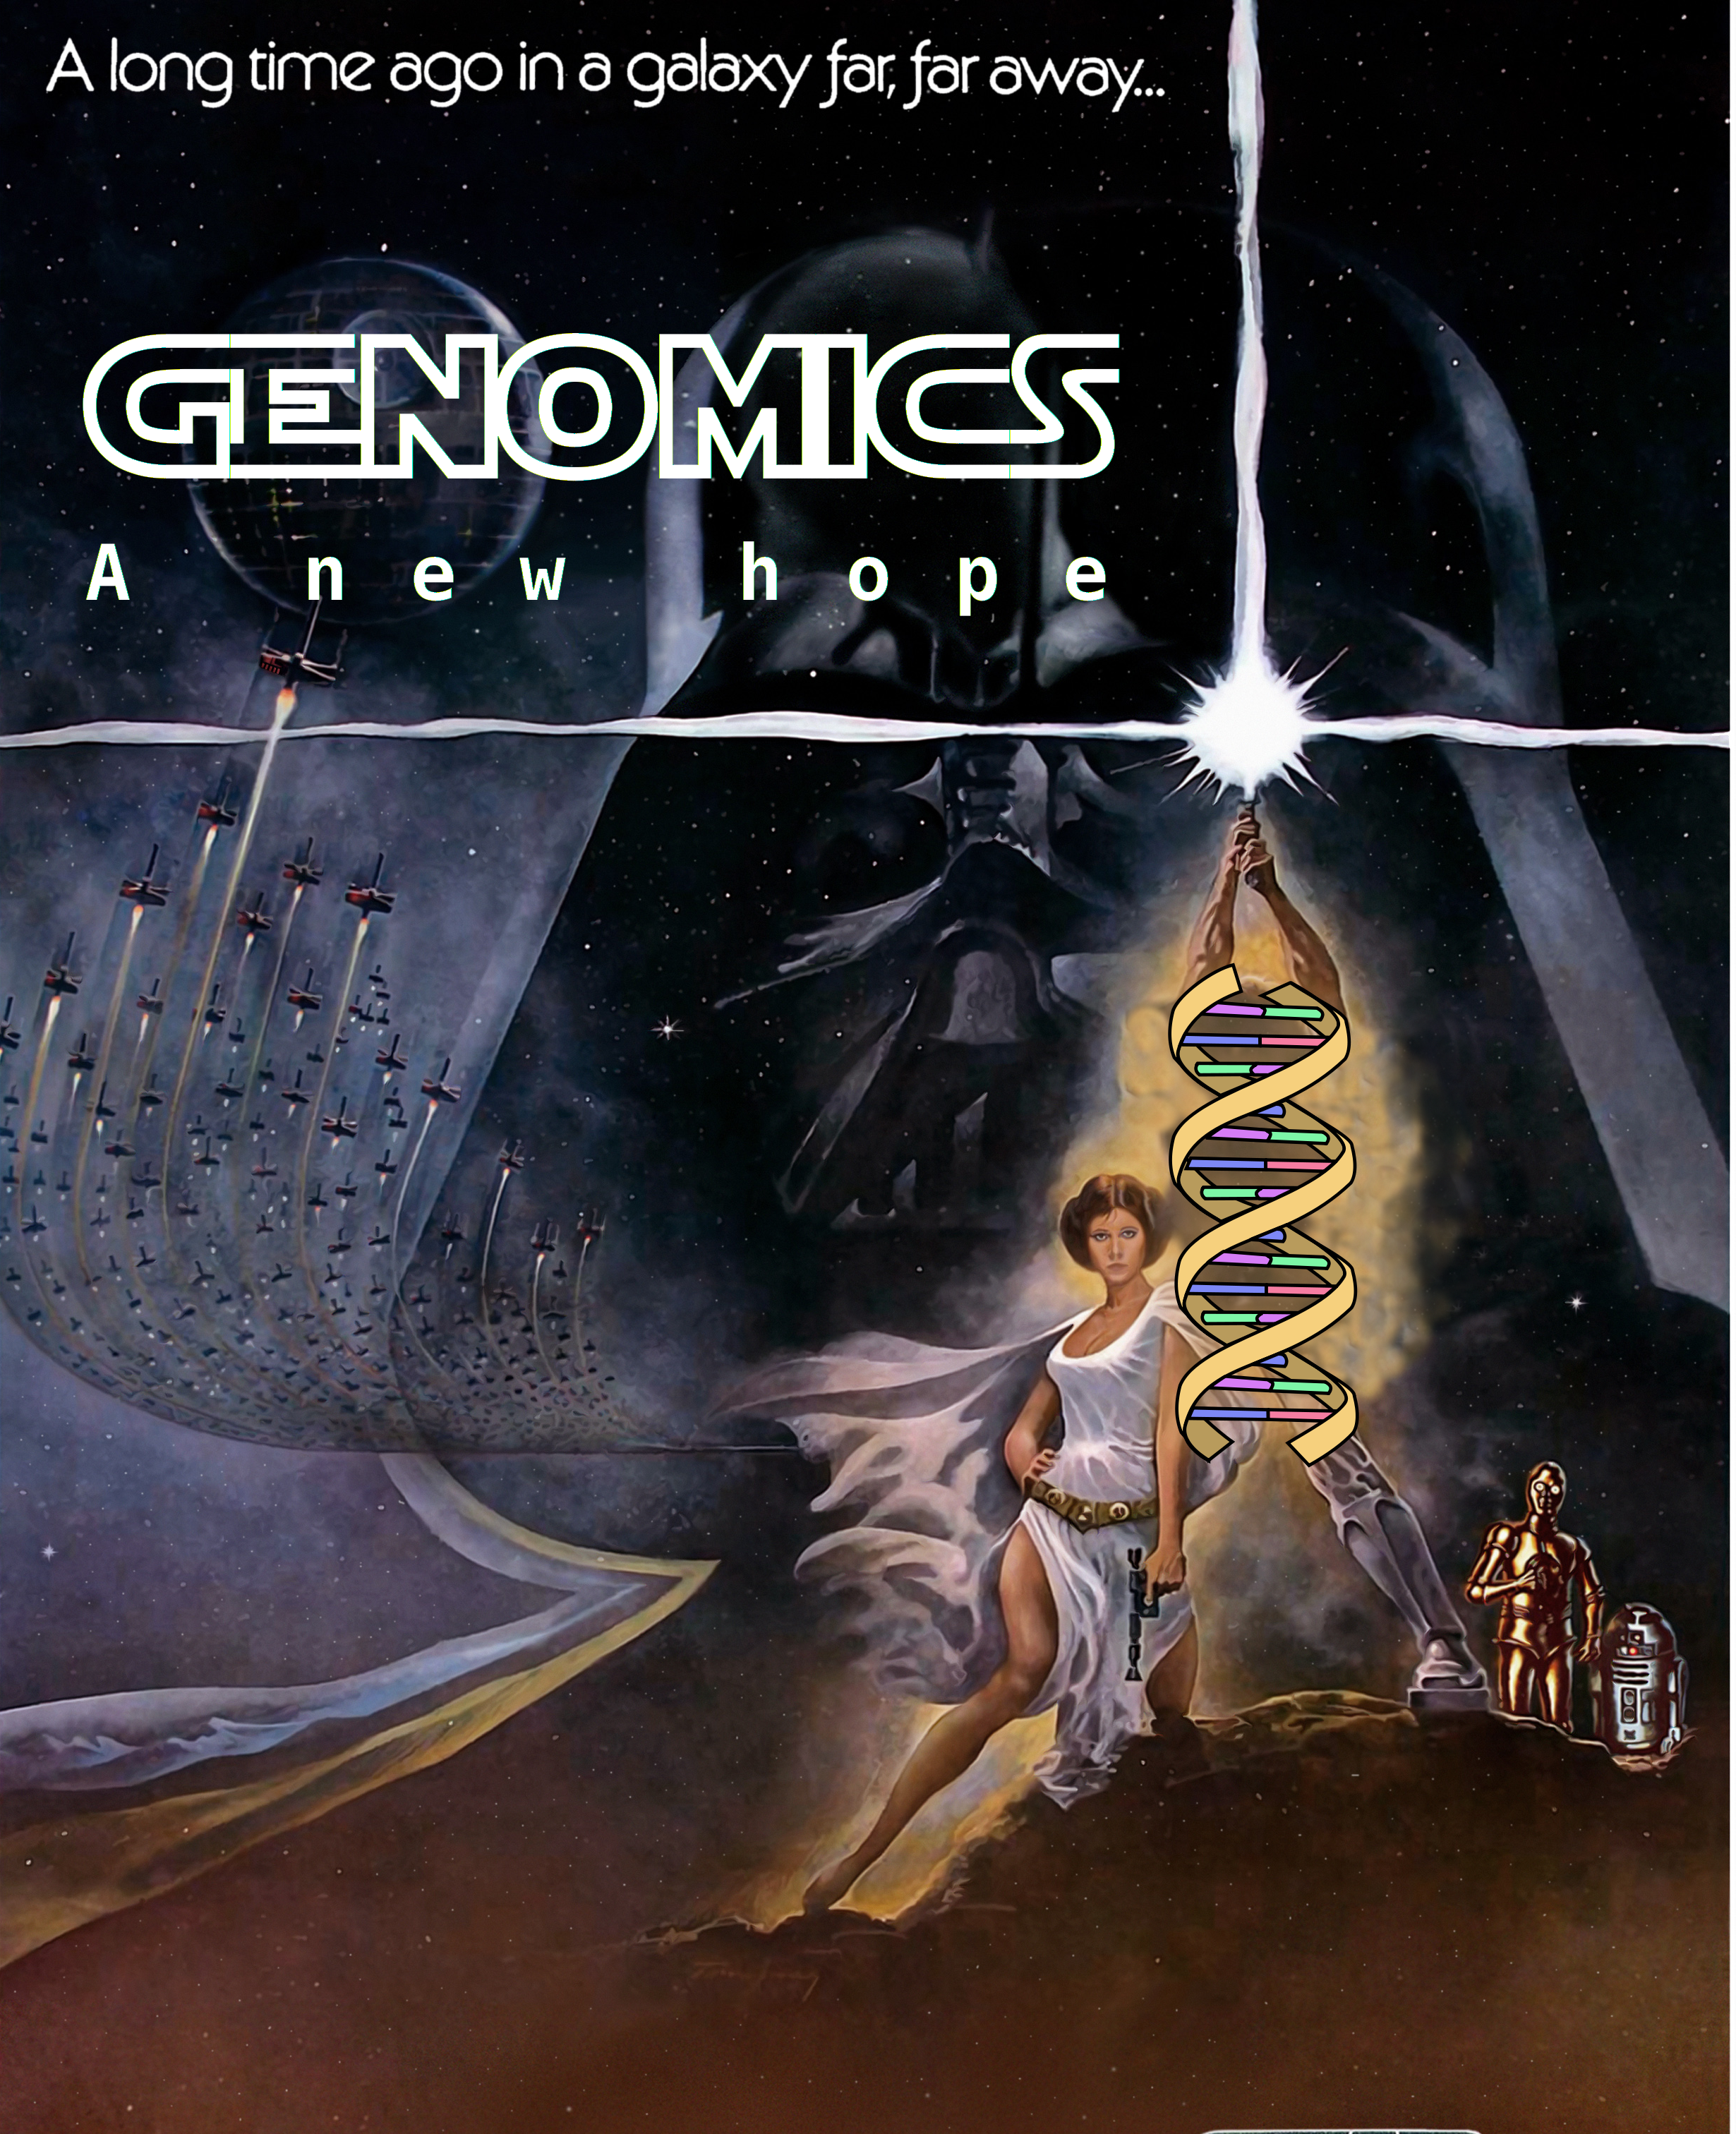
\includegraphics[height=0.85\textheight]{genomicsanewhopelow}}
\end{frame}
\note[itemize]{ \normalsize
\item The invention in 1977 of Sanger-based DNA sequencing3 which revolu-
tionised all branches of the biological sciences, could not be used for environmental bulk
samples because they contained potentially thousands of species, and separating them for
sequencing was prohibitively difficult.

\item It enabled the development of Barcoding => identifiying species by small segment of slow varying dna => Build taxonomic libraries based on barcodes

\item NGS method of high-throughput multi species identification using degraded
DNA found in the environment (

\item Costs went down by orders of magnitude and made DNA sequencing available to ecological studies}
\begin{frame}
	\frametitle{\LARGE Genomics; A new hope?}
	\begin{columns}
		\column{0.25\textwidth}
		\begin{center}
			\includegraphics[width=\textwidth]{samplingfromenvironment}
			Sampling from the Environment and Isolating the DNA
		\end{center}
		\column{0.25\textwidth}
		\uncover<2->{\centering
			\uncovergraphics<2->[width=\textwidth]{selectingprimers}   	
			Selecting appropriate primers   	
		}
		
		\column{0.25\textwidth}
		\uncover<3->{\centering
			\uncovergraphics<3->[width=\textwidth]{sequencing}  
			Sequencing DNA metabarcoding libraries 	
		}
		\column{0.25\textwidth}
		\uncover<4->{\centering
			\uncovergraphics<4->[width=\textwidth]{taxonomicidentification}   	
			OTU clustering and taxonomic identification
		}
	\end{columns} 
\end{frame}

\begin{frame}
	\frametitle{\Large Operational Taxonomic Units}
	\includegraphics[width=\textwidth]{otu}
\end{frame}
\note{
Sequncing => OTUs; genetic proxies for species. Sequences clustered with 97\% similarity and are given a signle otu name and taxonomy. Number of sequences in an OTU read => read counts}
	
	
	\section{Data}
		\begin{frame}
			\frametitle{Sampling}
			\setbeamertemplate{itemize/enumerate body begin}{\Large}
			
			\only<1,4->{\begin{itemize}
				\item<1-> Collected 164 samples from Northern Peruvian rivers
				
				\item<4-> Sequenced using Next generation sequencing 
				\item<5-> 675 OTUs matched with taxonomies from reference libraries
				\item<6-> Discarded the rest
				\item<7-> Recorded colour of water and location
			\end{itemize}}   
			\only<2>{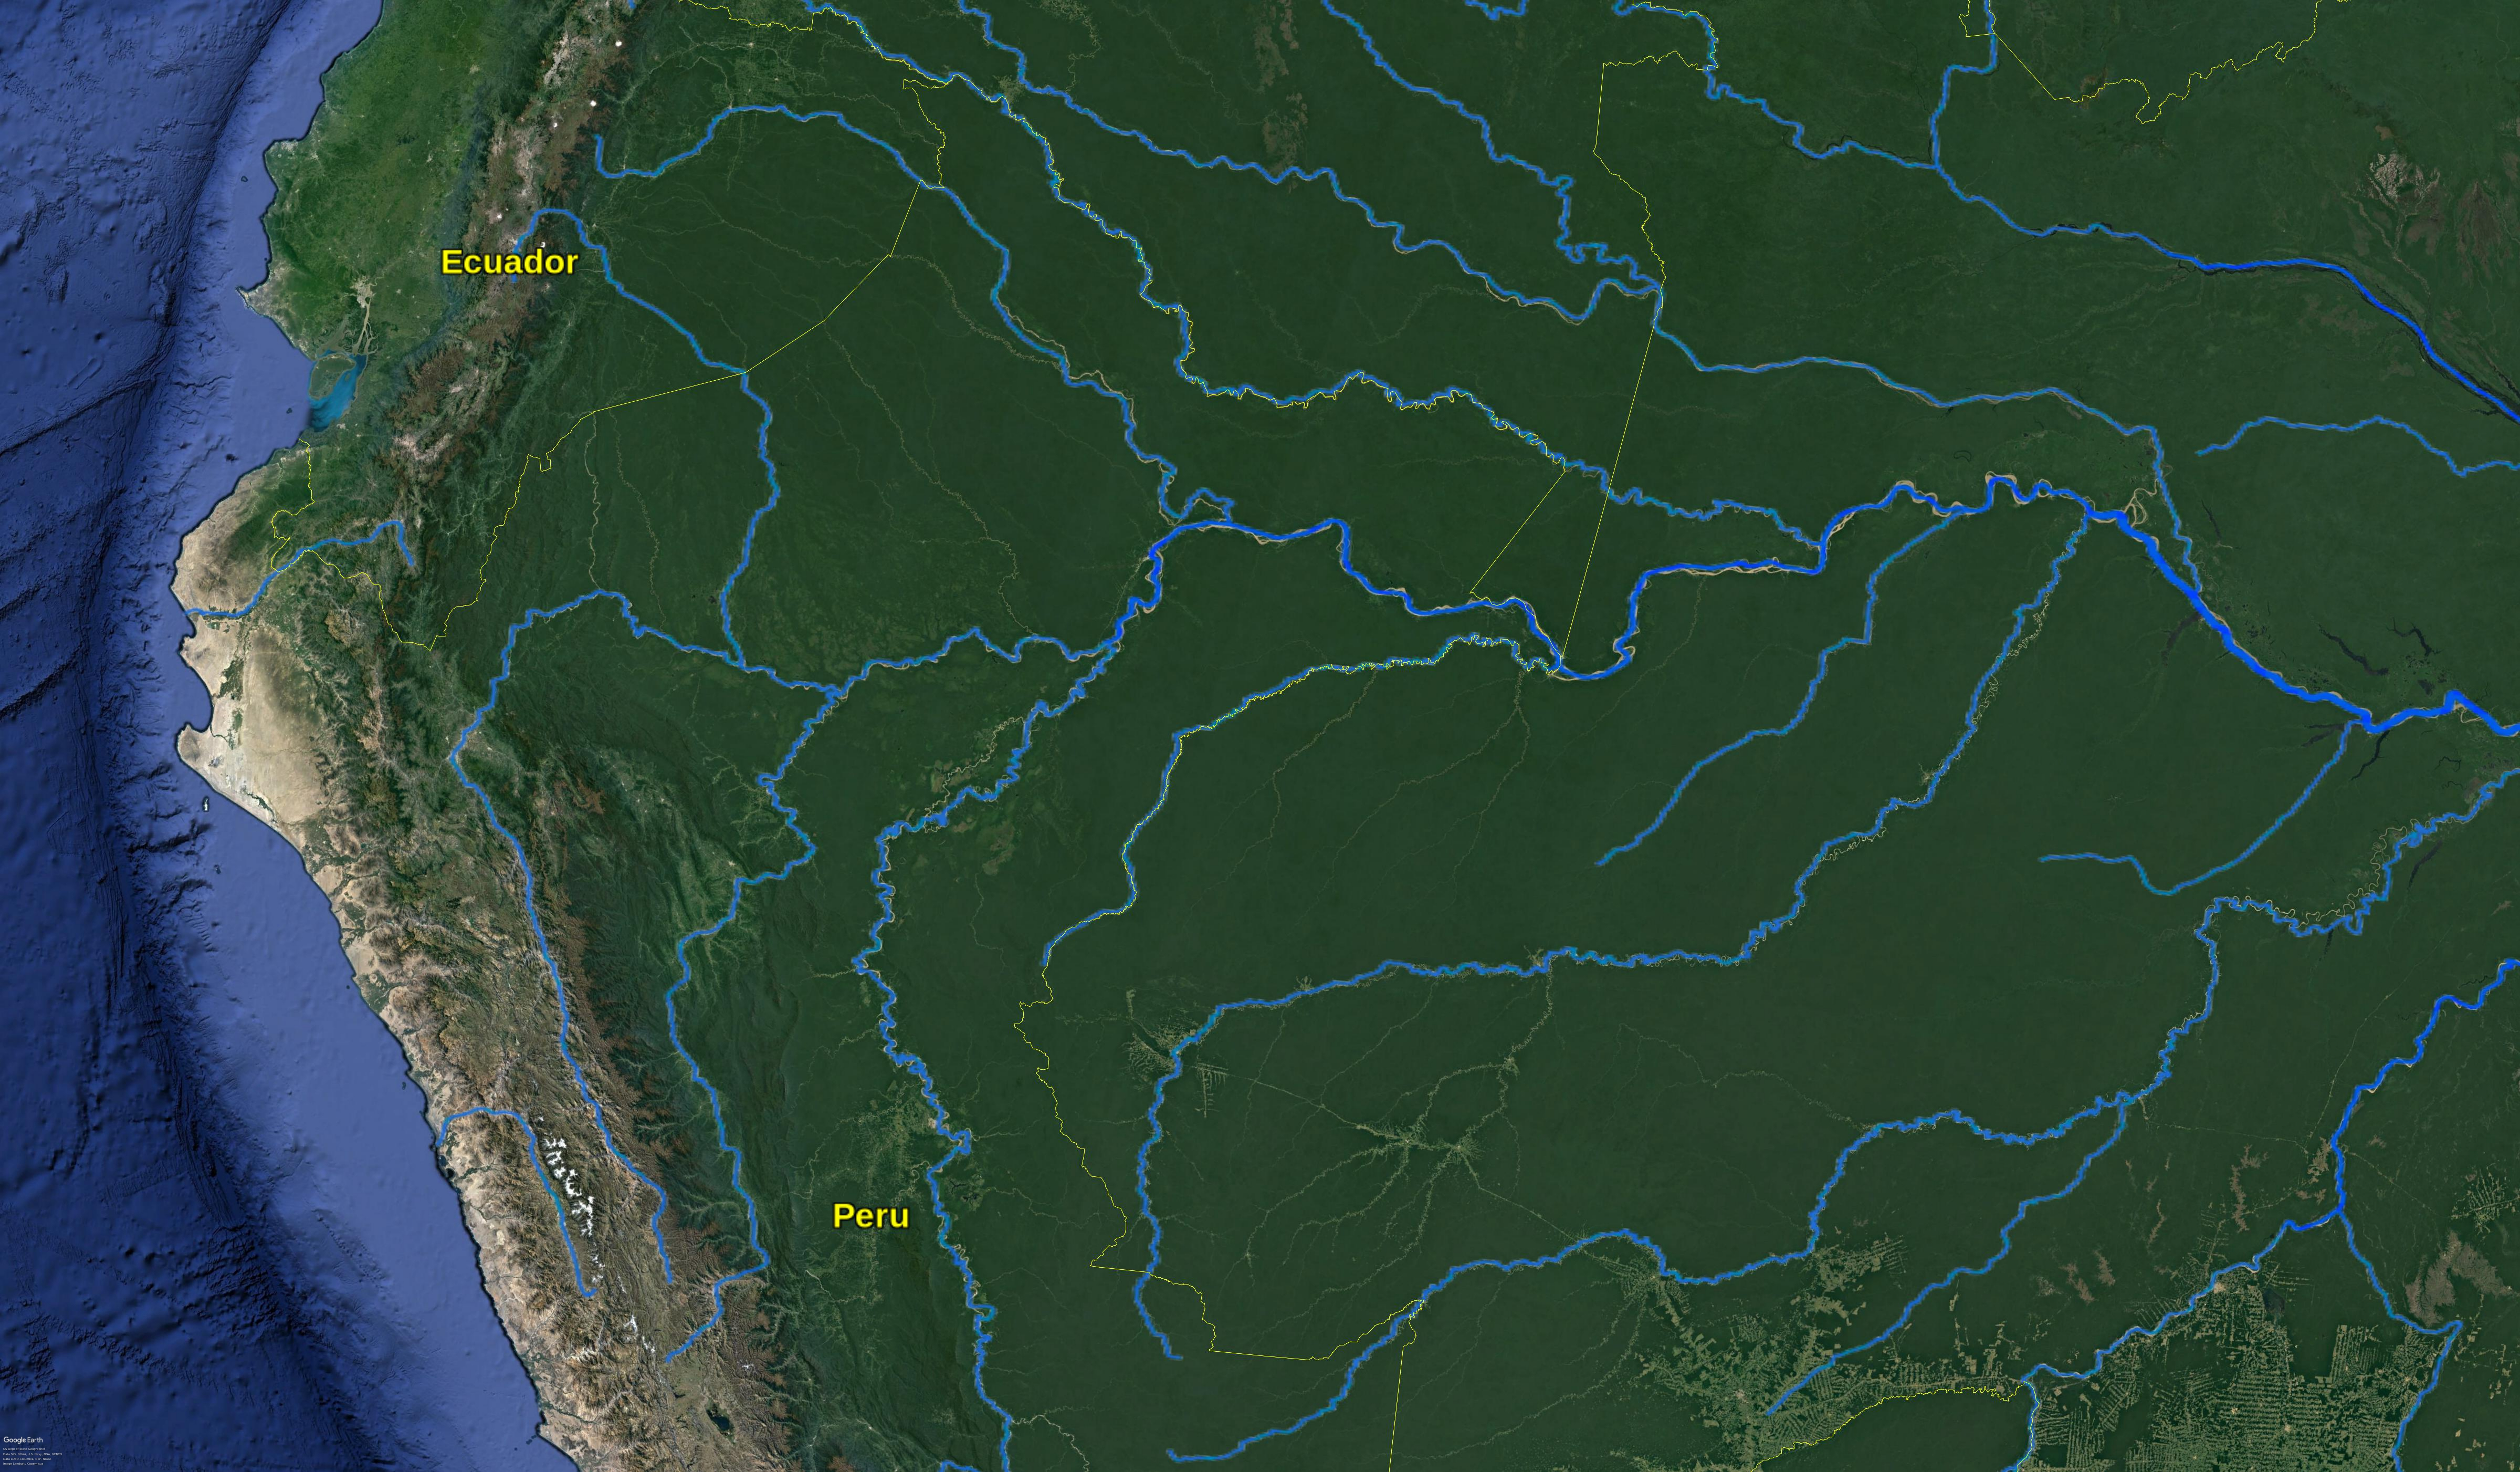
\includegraphics[width=\textwidth]{map1}}
			\only<3>{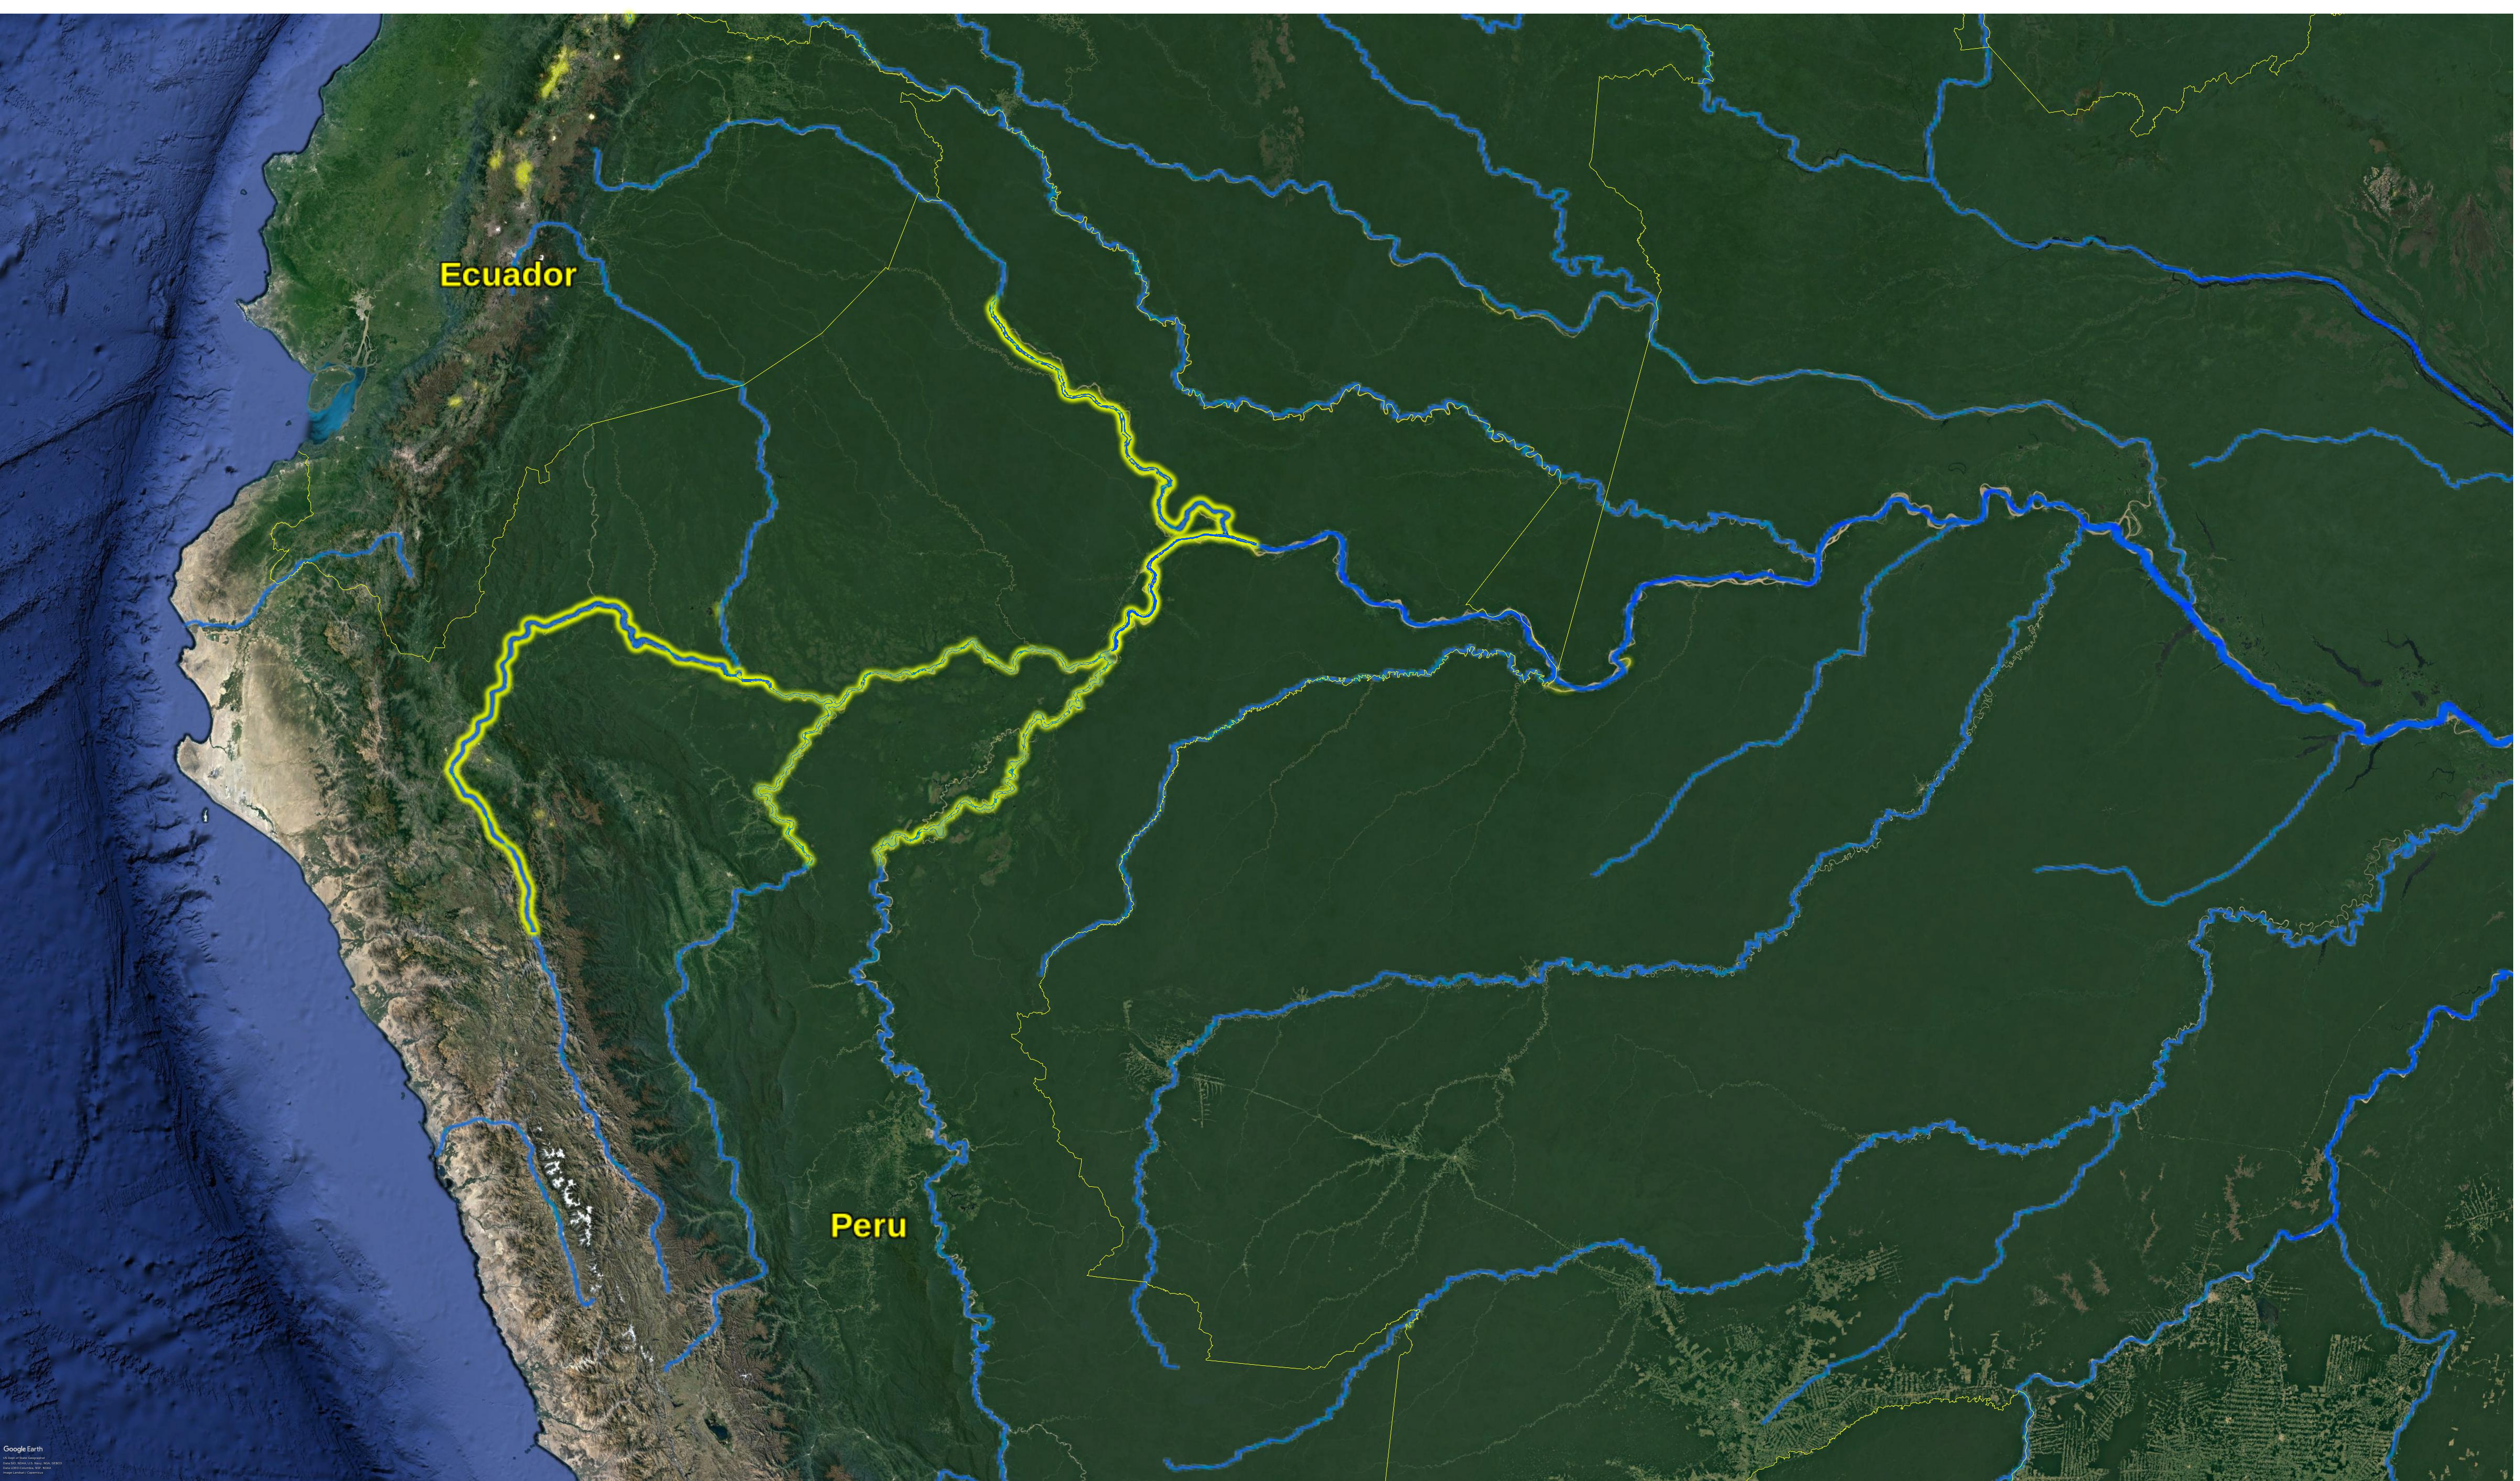
\includegraphics[width=\textwidth]{selectedrivers}}
		\end{frame}
\note[itemize]{\large
\item Collected 164 samples from northern peruvian rivers
\item The rivers can be seen in this photo highlighted by the yellow colour
\item Most abundand sequences in each otu were matched with a taxonomy. OTUs without one where discarded
\item
\item We also collected metadata about each sample. This included water colour and location of the sample}
\begin{frame}
	\frametitle{Meta Data}
	
	\only<1>{\centering
		\includegraphics[width=0.8\textwidth]{blackwhite}
	\\ White vs Black}
	\only<2>{\centering
	\includegraphics[width=\textwidth]{mapofrivers}}	
	
\end{frame}
\note[itemize]{
\item This is an example of Black and white water in the amazon. Essentially coffee with and without milk. Different concentration of minerals will inevitably lead to different species inhabitting the waters. It is our response variable; Can we predict water colour from species composition?
\item Unbalanced data set;143 white 21 black, most black water samples in the east}
		\begin{frame}
			\frametitle{Features}
			\only<1-7>{\begin{itemize}
				\item<+-> Sparse data matrix
				\item<+-> Dimensionality reduction  
				\begin{itemize}
					\item<+-> Principle Components Analysis
					\item<+-> Principle Coordinates Analysis \footfullcite{torgerson_multidimensional_1952}
					\item<+-> Non-metric Multidimensional Scaling \footfullcite{kruskal_multidimensional_1964}
					\item<+-> High spearman correlation features removed 
				\end{itemize}
	 		\item<+-> Cumulative sum scaling normalisation  and log transformation \footfullcite{css_diff_abund}
			\end{itemize}}
		\only<8>{\centering \includegraphics[height= 0.7\textheight]{histogramofcountdata}}
		\only<9>{\centering \includegraphics[height=0.7\textheight]{histogramofcountdatacss}}
		\only<10>{\centering \includegraphics[height= 0.7\textheight]{histogramofcountdatacsslog}}
		\end{frame}
\note[itemize]{\large
\item Ended up with 164 samples and a totla of 675 OTUs. Sparse matrix mostly zeroes. Thought appropriate to use dimensionality reduction
\item used oridnation methods => common in ecology for uncovering patterns in data
\item Principal components analysis finds axis with max variance and then orthogonal with second most
\item PCoA is generalisation of PCA. We can calculate dissimilarities between samples using distance metrics other than euclidean and then perform eigenanalysis on the distance matrix of the samples rather than covariance matrix. Used bray curtis commonly used in ecological studies. 
}\note[itemize]{\item nmds preserves order relations in dissimilarities between samples in the projection of data. EXAMPLE the  pairs of closest samples have to also be represented by the smallest interpoint distance in the ordination projection. 
\item high correlation
\item high variance in total read counts per sample. Used css normalisation (common method) to reduce variance. Log reduces further
}

\section{Train-Validation-Test}

		\begin{frame}
			\frametitle{Location and prediction}
			\only<1-3,5,7>{\begin{itemize}
				\item<+-> Location of train and test sets will affect performance of classifiers.
				\item<+-> Splitting data simulates different learning conditions .
				\item<+-> Maximally similar
				\item<5-> Maximally dissimilar
				\item<7> Random with equal distributions of black water in all sets
			\end{itemize}}
				\only<4>{\centering \includegraphics[height= 0.75\textheight]{stratsamp}}
				
				\only<6>{\centering \includegraphics[height= 0.75\textheight]{groupsamp2}}
		\end{frame}
\note[itemize]{\large
\item TEsting the classifiers will be affected by the location of the samples in the training and test sets. 
\item Splitting the data set in different ways is akin to testing the classifiers under different consitions
\item e.g. In maximally similar setting we simulate testing the models in geographical regions they have already seen
\item In maximaly dissimilar, we do the exact opposite by isolating the test from train
\item we also tried random sampling}

		\begin{frame}
			\frametitle{Model evaluation}
			\begin{itemize}
				\item<+-> Split data into train and test sets.
				\item<+-> Cross-validate model on validation sets created from train sets using the same principle as in train-test split; pick best hyperparameters based on accuracy.
				\item<+-> Test on the remaining samples in the test set.
				\item<+-> Repeat until all samples are found in the test set.

			\end{itemize}
		\end{frame}

		\begin{frame}
			\frametitle{Classifiers}
			\begin{itemize}
				\item<+-> Random Forest
				\item<+-> Logisitic regression with $L_1$ and $L_2$ penalty
				\item<+-> Bayesian Logistic Regression with Laplacian and Gaussian priors
			\end{itemize}
		\end{frame}
	
	%RESULTS%%%%%
	%%%%%%%%%%%%%
	%%%%%%%%%%%%%
	\section{Results}
		\begin{frame}
			\frametitle{Evaluating performance}
\begin{itemize}
	\item<1-> Can not use F score or ROC based on black water samples
	\item<2-> Some validation sets do not contain any black waters so most measures are undefined. Accuracy picks better models than F score based on white water.
\end{itemize}
\pause
\pause
\Large
Results presented in confusion matrix and accuracy:
\normalsize
\begin{equation}
\centering
\begin{bmatrix}
\text{Black samples Predicted correctly}&\text{Black samples Predicted falsely}\\
\text{White samples Predicted falsely}&\text{White  samples Predicted correctly}
\end{bmatrix}
\end{equation}
\end{frame}

\begin{frame}
	\frametitle{Best of Maximally similar}
  %	\setbeamertemplate{footline}{\vspace{0pt}}
	\setbeamertemplate{footline}{}
	\fontsize{9pt}{11}\selectfont
	\setlength\tabcolsep{3pt}
	\begin{tabular}{l c  c c}
		\toprule
		&\multicolumn{2}{c}{Confusion Matrix} & Accuracy\\
		Features used & Predicted Black&Predicted White&\\
		\midrule
		\rowcolor{LightPink} &19 &2&\\
		\rowcolor{LightPink} \multirow{-2}{*}{LR L1 OTU}&	 1&142&\multirow{-2}{*}{98.17\%}\\
		\cmidrule{2-3}
		\rowcolor{LightPink} &19 &2&\\
		\rowcolor{LightPink} \multirow{-2}{*}{LR L1 OTU LOW}&	 0&143&\multirow{-2}{*}{98.78\%}\\
		\cmidrule{2-3}
		\rowcolor{LightPink}&18 &3&\\
		\rowcolor{LightPink} \multirow{-2}{*}{LR L1 OTU CSS}&	 0&143&\multirow{-2}{*}{98.17\%}\\
		\cmidrule{2-3}
		\rowcolor{LightPink}
		&19 &2&\\
		\rowcolor{LightPink} \multirow{-2}{*}{LR L1 OTU CSS LOG}&	 1&142&\multirow{-2}{*}{98.17\%}\\
		\cmidrule{2-3}
		\rowcolor{LightPink}
		&20 &1&\\
		\rowcolor{LightPink} \multirow{-2}{*}{LR L2 OTU CSS LOG}&	 1&142&\multirow{-2}{*}{98.78\%}\\
		
		\cmidrule{2-3}
		\rowcolor{LightCyan}
		 &18 &3&\\
		\rowcolor{LightCyan} \multirow{-2}{*}{RF OTU LOW}&	 3&140&\multirow{-2}{*}{96.34\%}\\
		
		\cmidrule{2-3}
		\rowcolor{LightCyan}
		 &18 &3&\\
		\rowcolor{LightCyan} \multirow{-2}{*}{RF OTU CSS}	&	 3&140&\multirow{-2}{*}{96.34\%}\\
	
		\cmidrule{2-3}
		\rowcolor{LightCyan}
		 &19 &2&\\
		\rowcolor{LightCyan} \multirow{-2}{*}{RF OTU CSS LOG}&	 3&140&\multirow{-2}{*}{96.95\%}\\
		\bottomrule
	\end{tabular}
\end{frame}	
\begin{frame}
	\frametitle{Most important taxonomic orders}
	\begin{columns}
		\column{0.5\textwidth}
		\centering
		\includegraphics[width=\textwidth]{rfr_sim_mean_pieOTU CSS LOG}		
		Aggregating importance by averaging over Order
		\column{0.5\textwidth}
		\centering
		\includegraphics[width=\textwidth]{rfr_sim_sum_pieOTU CSS LOG}		
				Aggregating importance by summing over Order
	\end{columns}
\end{frame}


\begin{frame}
\frametitle{Most important taxonomic orders}
\begin{columns}
	\column{0.5\textwidth}
	\includegraphics[width=\textwidth]{tapir}
	South American Tapir\footnotemark		
	\column{0.5\textwidth}
	\includegraphics[width=\textwidth]{pinkdolphin}
	Amazon river dolphin\footnotemark 
\end{columns}
\footnotetext[1]{\fullcite{charles_tapir_2019}} 
\footnotetext[2]{\fullcite{pinkdolphin}}		
\end{frame}


\begin{frame}
		\frametitle{Best of Maximally Dissimilar}
		 \setbeamertemplate{footline}{\vspace{0pt}}
		\fontsize{11pt}{13}\selectfont
		\setlength\tabcolsep{3pt} 
		
			\begin{tabular}{l c  c c}
			\toprule
			&\multicolumn{2}{c}{Confusion Matrix} & Accuracy\\
			Features used & Predicted Black&Predicted White&\\
\midrule
			\rowcolor{LightPink}
			 &8 &13&\\
			\rowcolor{LightPink} \multirow{-2}{*}{L1 PCoA CSS 99\%}&	 5&138&\multirow{-2}{*}{89.02\%}\\	
			\cmidrule{2-3}
			\rowcolor{LightPink}
			 &7 &14&\\
			\rowcolor{LightPink} \multirow{-2}{*}{L1 PCoA 90\%}&	 5&138&\multirow{-2}{*}{88.41\%}\\
			\cmidrule{2-3}
		\rowcolor{LightPink}	
			&12 &9&\\
		\rowcolor{LightPink}			\multirow{-2}{*}{L2 OTU CSS LOG}&	 1&142&\multirow{-2}{*}{93.90\%}\\
			\cmidrule{2-3}
		\rowcolor{LightCyan}			
			&7 &14&\\
		\rowcolor{LightCyan}			\multirow{-2}{*}{RF OTU CSS LOG}&	 2&141&\multirow{-2}{*}{90.24\%}\\
		\cmidrule{2-3}				
			\rowcolor{LightCyan}
			&7 &14&\\
			\rowcolor{LightCyan}
			\multirow{-2}{*}{RF OTU CSS}&	 2&141&\multirow{-2}{*}{90.24\%}\\
			\bottomrule
		\end{tabular}
\end{frame}

\begin{frame}
	\frametitle{Bayesian Logistic Regression}
		\setbeamertemplate{footline}{}
	\fontsize{9pt}{11}\selectfont
	\setlength\tabcolsep{6pt}
				\setbeamertemplate{itemize/enumerate body begin}{\large}
	\begin{itemize}
		\item<+-> Sampling is very slow and poor when using any OTU or PCoA features.
		\item<+-> Only works with 20 dimensions of NMDS
		\item<+-> Produces better results than Maximum Likelihood version of Logistic Regression using same feature set
	\end{itemize}
	\centering

	\onslide<+->{ \begin{tabular}{l c  c c}

	\toprule
	&\multicolumn{2}{c}{Confusion Matrix} & Accuracy\\
	Features used & Predicted Black&Predicted White&\\
	\midrule
	\multirow{2}{*}{Max. Sim. NMDS $L_1$} &13 &8&\multirow{2}{*}{95.12\%}\\
	&	0&143&\\
	\cmidrule{2-3}
	\multirow{2}{*}{Max. Sim. NMDS $L_2$} &8&13&\multirow{2}{*}{92.07\%}\\
	&	0&143&\\
		\multirow{2}{*}{Max. Dissim. NMDS $L_1$} &3 &18&\multirow{2}{*}{83.54\%}\\
	&	9&134&\\
	\cmidrule{2-3}
	\multirow{2}{*}{Max. Dissim. NMDS $L_2$} &0&21&\multirow{2}{*}{92.07\%}\\
	&	21&140&\\
	\bottomrule
\end{tabular}}

\end{frame}
\begin{frame}
	\frametitle{Conclusions}
	\begin{itemize}
	\item<+-> Maximum Dissimilarity is a harder setting than similarity for prediction
	\item<+-> CSS normalisation and Log transformation produce the best feature set. Ordination methods may not be useful.
	\item<+-> Only a small set of taxonomic Orders are contributing to prediction
	\item<+-> Between Random Forest and Logistic regression there is no significant difference in predictive ability.
	\item<+-> Bayesian methods are promising but slow
	\end{itemize}
\end{frame}
	\appendix
	
	\backupbegin
%	\section{Extra Slides}
	\begin{frame}
		\frametitle{Ordination Plots}
		\only<1>{\centering
			PCA
			\includegraphics[height=0.75\textheight]{pcaotu12}}
		\only<2>{\centering
			PCoA
			\includegraphics[height=0.75\textheight]{pcoaotu12}}
		\only<3>{\centering
		NMDS
		\includegraphics[height=0.75\textheight]{nmdsotu12}}
	\end{frame}
	\begin{frame}
	\frametitle{Benchmark}
		\centering
		\begin{tabular}{l c c c}
		\toprule 
		&\multicolumn{2}{c}{Confusion Matrix} &Accuracy\\
		Features used & Predicted Black&Predicted White&\\ 
		
		\midrule
		\multicolumn{4}{c}{Maximum Similarity}\\
		\cmidrule{1-4}
		\multirow{2}{*}{All Labels }& 	2.64 & 18.36&		\multirow{2}{*}{77.6\%}\\
		&	18.36 &124.64&\\
		\cmidrule{2-3}
		\multirow{2}{*}{Min Labels}  &2.75 & 18.25&		\multirow{2}{*}{76.8\%}\\
		&18.25& 117.75&\\
		\cmidrule{1-4}
		\multicolumn{4}{c}{Maximum Dissimilarity}\\ 
		\cmidrule{1-4}
		\multirow{2}{*}{All Labels }&  1.75 &19.25&\multirow{2}{*}{76.7\%}\\
		&	 18.96&124.04 &\\
		\cmidrule{2-3}
		\multirow{2}{*}{Min Labels}    &1.83&19.17&\multirow{2}{*}{75.8\% }\\
		&18.83&117.17&\\
		\bottomrule
	\end{tabular}	
\end{frame}
	  \begin{frame}
	    \frametitle{Maximally Similar LR}
	    \setbeamertemplate{footline}{\vspace{0.5pt}}
		\fontsize{12pt}{8}\selectfont
		\setlength\tabcolsep{3pt} 
		%\footnotesize
		\vspace{1cm}
	    	\centering
%	    	\caption{Results from maximising similarity using Logistic Regression}
	    	\label{table:lrsimilarity}
	    	\begin{tabular}{l c  c c}
	    		\toprule
	    		&\multicolumn{2}{c}{Confusion Matrix} & Accuracy\\
	    		Features used & Predicted Black&Predicted White&\\
	    		\midrule
	    		 &19 &2&\\
	    		\multirow{-2}{*}{OTU}&	 1&142&\multirow{-2}{*}{98.17\%}\\
	    		\cmidrule{2-3}
	    		\multirow{2}{*}{OTU LOW} &19 &2&\multirow{2}{*}{98.78\%}\\
	    		&	 0&143&\\
	    		\cmidrule{2-3}
	    		\multirow{2}{*}{OTU CSS}&18 &3&\multirow{2}{*}{98.17\%}\\
	    		&	 0&143&\\
	    		\cmidrule{2-3}
	    		\multirow{2}{*}{OTU Min CSS}&18 &3&\multirow{2}{*}{98.09\%}\\
	    		&	 0&136&\\
	    		\cmidrule{2-3}
	    		\multirow{2}{*}{OTU CSS LOG}&19 &2&\multirow{2}{*}{98.17\%}\\
	    		&	 1&142&\\
	    		\cmidrule{2-3}
	    		\multirow{2}{*}{PCoA Bray-Curtis} &16 &5&\multirow{2}{*}{95.12\%}\\
	    		&	 3&140&\\
	    		\cmidrule{2-3}
	    		\multirow{2}{*}{PCoA Bray-Curtis CSS} &16 &5&\multirow{2}{*}{96.34\%}\\
	    		&	 1&142&\\
	    		\bottomrule
	    	\end{tabular}
	\end{frame}


  	\begin{frame}
		\frametitle{Maximally Similar RF}
			\fontsize{12pt}{8}\selectfont
			\setlength\tabcolsep{3pt} 
			\vspace{1cm}	
				\centering
				\label{table:rfrsimilarity}
				\begin{tabular}{l c  c c}
					\toprule
					&\multicolumn{2}{c}{Confusion Matrix} & Accuracy\\
					Features used & Predicted Black&Predicted White&\\
					
					\midrule
					\multirow{2}{*}{OTU} &17 &4&\multirow{2}{*}{95.73\%}\\
					&	 3&140&\\
					\cmidrule{2-3}
					\multirow{2}{*}{OTU LOW} &18 &3&\multirow{2}{*}{96.34\%}\\
					&	 3&140&\\
					\cmidrule{2-3}
					\multirow{2}{*}{OTU CSS} &18 &3&\multirow{2}{*}{96.34\%}\\
					&	 3&140&\\
					\cmidrule{2-3}
					\multirow{2}{*}{OTU Min CSS}&18 &3&\multirow{2}{*}{96.18\%}\\
					&	 3&133&\\
					\cmidrule{2-3}
					\multirow{2}{*}{OTU CSS LOG} &19 &2&\multirow{2}{*}{96.95\%}\\
					&	 3&140&\\
					\cmidrule{2-3}
					\multirow{2}{*}{PCoA Bray-Curtis} &6 &15&\multirow{2}{*}{88.41\%}\\
					&	 4&139&\\
					\cmidrule{2-3}
					\multirow{2}{*}{PCoA Bray-Curtis CSS} &4 &17&\multirow{2}{*}{89.63\%}\\
					&	 0&143&\\
					\bottomrule
				\end{tabular}	
	\end{frame}


	\begin{frame}{Maximally Dissimilar LR}
	  	\setbeamertemplate{footline}{\vspace{0.5pt}}
	\fontsize{12pt}{8}\selectfont
	\setlength\tabcolsep{3pt}
	\centering
		\begin{tabular}{l c  c c}
		\toprule
		&\multicolumn{2}{c}{Confusion Matrix} & Accuracy\\
		Features used & Predicted Black&Predicted White&\\
		\midrule
		\multirow{2}{*}{OTU} &5 &16&\multirow{2}{*}{79.27\%}\\
		&	 18&125&\\
		\cmidrule{2-3}
		\multirow{2}{*}{OTU LOW} &5 &16&\multirow{2}{*}{79.88\%}\\
		&	 17&126&\\
		\cmidrule{2-3}
		\multirow{2}{*}{OTU CSS}&7 &14&\multirow{2}{*}{82.93\%}\\
		&	 14&129&\\
		\cmidrule{2-3}
		\multirow{2}{*}{OTU Min CSS}&3 &18&\multirow{2}{*}{79.61\%}\\
		&	 14&122&\\
		\cmidrule{2-3}
		\multirow{2}{*}{OTU CSS LOG}&5 &16&\multirow{2}{*}{87.80\%}\\
		&	 4&139&\\
		\cmidrule{2-3}
		\multirow{2}{*}{PCoA Bray-Curtis} &7 &14&\multirow{2}{*}{86.59\%}\\
		&	 8&135&\\
		\cmidrule{2-3}
		\multirow{2}{*}{PCoA Bray-Curtis CSS} &9 &12&\multirow{2}{*}{87.80\%}\\
		&	 8&135&\\
		\bottomrule
	\end{tabular}
	
\end{frame}

%MAX DIS RF
	\begin{frame}{Maximally Dissimilar RF}
\setbeamertemplate{footline}{\vspace{0.5pt}}
\fontsize{12pt}{8}\selectfont
\setlength\tabcolsep{3pt}
\centering
\begin{tabular}{l c  c c}
	\toprule
	&\multicolumn{2}{c}{Confusion Matrix} & Accuracy\\
	Features used & Predicted Black&Predicted White&\\
	\midrule
	\multirow{2}{*}{OTU} &4 &17&\multirow{2}{*}{83.50\%}\\
	&	 10&133&\\
	\cmidrule{2-3}
	\multirow{2}{*}{OTU LOW} &2&19&\multirow{2}{*}{82.32\%}\\
	&	 10&133&\\
	\cmidrule{2-3}
	\multirow{2}{*}{OTU CSS}&7 &14&\multirow{2}{*}{90.24\%}\\
	&	 2&141&\\
	\cmidrule{2-3}
	\multirow{2}{*}{OTU Min CSS}&7 &14&\multirow{2}{*}{90.45\%}\\
	&	 1&135&\\
	\cmidrule{2-3}
	\multirow{2}{*}{OTU CSS LOG}&7 &14&\multirow{2}{*}{90.24\%}\\
	&	 2&141&\\
	\cmidrule{2-3}
	\multirow{2}{*}{PCoA Bray-Curtis} &0 &21&\multirow{2}{*}{86.59\%}\\
	&	 1&142&\\
	\cmidrule{2-3}
	\multirow{2}{*}{PCoA Bray-Curtis CSS} &0 &21&\multirow{2}{*}{84.15\%}\\
	&	 5&138&\\
	\bottomrule
\end{tabular}


\end{frame}
	\backupend

\end{document}